\documentclass{report}
\usepackage{graphicx}
\usepackage{hyperref}
\usepackage{rotating}

\author{Luke Maurits, \\
Add your name here, \\
If you contribute material, \\
Use alphabetical order}
\title{CLLARE Project Overview}
\begin{document}
\maketitle
\tableofcontents

\chapter{Introduction}

\section{What is CLLARE?}

The Collaborative Lunar Landing and Research Expedition (CLLARE) project is a proposed spaceflight project with the goal of landing a single human on the moon and returning them safely to Earth.  By using a reduced crew size, modern technology and a design philosophy emphasising simplicity and reusability, CLLARE endeavours to be an extremely low-cost project in comparison to Apollo or Constellation.

CLLARE is an ``open source'' spaceflight project.  What does this mean?  It means that documents such as this one and others which describe CLLARE in intimate technical detail, including spreadsheets and CAD files, are available for free under the Creative Commons Attribution Sharealike 3.0 license, so that anybody can copy, distribute and modify them.  It means that computer code to handle every aspect of planning and running CLLARE is available for free under the GNU General Public License 3,0, so that anybody can copy, distribute and modify it.  Anybody who has the desire, determination and money can build and launch the CLLARE hardware without any fear of legal issues (at least not from the people who planned CLLARE - some countries may have restrictions on who can launch what into space, when and where).  It means that anybody with the interest and knowledge can help refine the CLLARE project.

\section{Who is organizing CLLARE?}

CLLARE is a project of the Collaborative Space Travel and Research Team (CSTART).  CSTART is a non-government, non-profit space agency run by volunteers.  It provides online services to facilitate the planning and promotion of open source projects related to space travel and space research, like CLLARE.  It also attempts to raise the money required to fund these projects, or at least to fund the construction of proof--of--concept mock ups.  In the future CSTART may organize and fund space travel and research related prizes, with the condition that all entries are released under open source licenses at the end of the competition.

\section{How can I get involved in CLLARE?}

\section{How can I suggest changes/corrections/improvements to this document?}

%%%%%%%%%%%%%%%%%%%%%%%%%%%%%%%%%%%%%%%%%%%%%%%%%%

\chapter{Project Overview}

\section{Mission Overview}

The CLLARE mission is based around a Lunar Orbit Rendezvous (LOR) structure.  A spacecraft composed of several connected modules is launched into a low Earth ``parking orbit'', using a multiple stage rocket booster.  Following successful completion of various checks and tests, a Trans Lunar Injection (TLI) burn is performed, taking the spacecraft out of LEO and putting it on a lunar free return trajectory: a trajectory such that, with no further changes in velocity, the craft will travel close enough to the moon for the moon's gravitational field to cause reversal in its direction, putting it on a return course for Earth.  This choice of trajectory is an important safety feature for CLLARE.

Once the spacecraft is sufficiently close to the moon, a Lunar Orbit Insertion (LOI) or ``lunar capture'' burn slows the spacecraft down to such a speed that it enters a low lunar orbit.

Lander descent and ascent happens here.

Once the lunar rendezvous has been completed, a Trans Earth Injection (TEI) or ``lunar escape'' burn accelerates the spacecraft to a sufficiently high speed to escape the moon's gravitational field, leaving it on a course bound for Earth.

Atmospheric reentry happens here.

\section{Core CLLARE Hardware}

The CLLARE project is based around a set of modular hardware items, referred to as the core CLLARE hardware.  By combining items from the core hardware in appropriate configurations, a number of different mission types can be flown.  This approach allows a gradual progression toward the ultimate lunar goal.

The sections below introduce the core hardware items.  Figure \ref{fig:cm_configs} shows the various configurations of the hardware.  Chapter \ref{chap:detailed} describes more detailed descriptions of each hardware item and its subsystems, including diagrams.

\subsection{The CLLARE Command Module}

The \href{http://cstart.org/wiki/CLLARE_Command_Module}{CLLARE Command Module} (CM) is a one-person spacecraft in the ``truncated cone and cylindrical nose'' shape of the Mercury and Gemini spacecraft, which strongly influenced its design.  The CM contains sufficient onboard supplies of all required consumables to support its occupant for a duration of 24 hours, including support for one repressurisation of the capsule after extra vehicular activity (EVA) via an ingress-egress hatch.  An ablative heat shield permits the CM to reenter the Earth's atmosphere.  The CM will be capable of landing in water and possible also on land.  Suggested landing options include parachute, paraglider and ballute.  The CM will be designed to be as reusable as possible.

As a stand alone unit, the CM is capable of supporting only suborbital flights, making it functionally equivalent to early (suborbital) flights of the US Mercury craft.  More ambitius flights, including lunar landing missions, are facilitated by the use of a family of attachable modules.

\subsection{The CLLARE Retro Module}

The \href{http://cstart.org/wiki/CLLARE_Retro_Module}{CLLARE Retro Module} (RM) is a small, cylindrical module which attaches to the rear of the CLLARE CM.  The module contains a set of small and simple rockets (either solid or hybrid fuelled).  The module facilitates the use of the CM for orbital flights, by providing the means to deorbit such a CM.  The manner in which the RM attaches to the rear of the CM is such that the two modules can be separated after a deorbit burn, prior to reentry.  The RM is not equipped to survive reentry and burns up in Earth's atmosphere.

A CLLARE CM-RM combination is functionally equivalent to later (orbital) flights of Mercury or, if EVA is performed, early flights of the US Gemini craft.

\subsection{The CLLARE Mission Extension Module}

The \href{http://cstart.org/wiki/CLLARE_Mission_Extension_Module}{CLLARE Mission Extension Module} (MEM) is a cylindrical module which attaches to the rear of the the CM.  The module contains sufficient supplies of all required consumables to extend the CM's standalone endurance of 24 hours to a total of 7 days.  Consumables are conveyed from the MEM to the CM through an umbillical system which penetrates the CM's heat shield in a controlled manner.

The rear end of the MEM is sufficiently similar to the rear end of the CM that a CLLARE Retro Module can be attached to it, facilitating long-duration orbital missions.  In this configuration the MEM and RM are detached as a single unit prior to reentry.  The MEM is not equipped to survive reentry and burns up along with the RM.

A CLLARE CM-MEM-RM combination is functionally equivalent to the later flights of Gemini.

\subsection{The CLLARE Propulsion Module}

The \href{http://cstart.org/wiki/CLLARE_Propulsion_Module}{CLLARE Propulsion Module} (PM) is a cylindrical module which attaches to the rear of a CLLARE Command Module or Mission Extension Module.  The module contains a set of propellant tanks and contains a liquid bipropellant rocket at its end.  The PM is able to provide large changes in velocity to a CM or CM-MEM combination, allowing high-altitude Earth orbital flights or circumlunar flights.  The PM can also be used to perform deorbit burns, replacing the Retro Module for flights using a PM.  The PM is not equipped to survive reentry and burns up along with any other modules.

A CLLARE CM-MEM-PM combination is functionally equivalent to an Apollo Command Module and Service Module (CSM) combination (with no docked Lunar Module) - the MEM-PM combination is roughly functionally equivalent to the the Apollo SM.

In principle, multiple MEMs and PMs could be combined behind a single CM to allow arbitrarily long and distant flights, but launching such combinations would eventually become infesible.

\subsection{The CLLARE Lunar Mission Module}

The \href{http://cstart.org/wiki/CLLARE_Lunar_Mission_Module}{CLLARE Lunar Mission Module} (LMM) is a large cylindrical module which attaches to the rear of a CM-MEM combination.  The module provides all the facilities required to facilitate a lunar landing mission.  It includes a set of propellant tanks similar in design to those of the Propulsion Module, but larger (to support additional lunar capture and lunar escape burns) and space for the CLLARE Lunar Lander (see below) to dock.  Two ideas have been proposed for propulsion: in one, the LMM has a cluster of engines at its end, these engines being identical to thoseused on the PM; in the other, the Lunar Lander's engine (which is also identical to the PM engine) is used to provide propulsion.

A CLLARE CM-MEM-LMM combination is functionally equivalent to the full Apollo Spacecraft (i.e. Command Module, Service Module and Lunar Module).

\subsection{The CLLARE Lunar Lander}

The \href{http://cstart.org/wiki/CLLARE_Lunar_Lander}{CLLARE Lunar Lander} (LL) is a light weight, open cabin lunar landing craft.  Unlike the Apollo lunar lander (and like the planned Soviet lunar lander), the LL is not composed of two separable stages.  The entire structure undergoes a lunar descent and a lunar ascent, with the same engine and set of fuel tanks used for both directions.  The lunar lander's engine is a liquid bipropellant rocket and is the same engine as used for the CLLARE Propulsion Module and some versions of the Lunar Mission Module.

\begin{figure}[h] \label{fig:cm_configs}
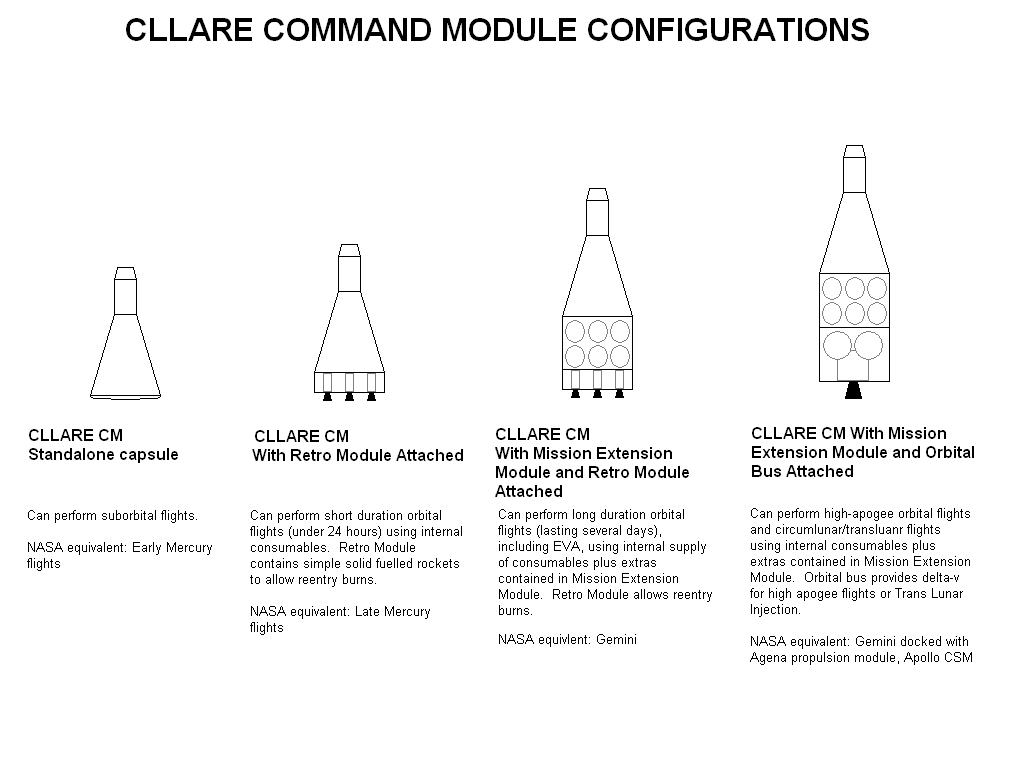
\includegraphics[angle=270, scale=0.6]{images/cllare_cm_configs}
\caption{Various configurations of the CLLARE core hardware (somewhat outdated).}
\end{figure}

\section{Launch Options}

\subsection{Suborbital and orbital missions}

The proposed suborbital and orbital flight configurations (CM and CM-OSM) have estimated total masses in the vicinity of 1,000 kg and 1,250 kg, respectively (see Chapter \ref{chap:numeric} for details of these estimates).

CSTART is not aware of any man--rated commercial launch vehicles designed to carry payloads of this mass, so is considering the development of its own launch capabilities for these missions.  The current plan of approach is to use variably sized clusters of small, simple and inexpensive rockets to lift payloads around 1,000 kg in mass into LEO, a concept pioneered by the \href{http://en.wikipedia.org/wiki/OTRAG}{OTRAG company} project in the 1970s.  We are keen to use hybrid rocket engines for the small rockets due to their high levels of safety and excellent trade-off between simplicity and performance.

A group called \href{http://www.copenhagensuborbitals.com/}{Copenhagen Suborbitals}, based in Denmark, are currently working on a hybrid rocket engine designed to perform suborbital flights for a manned, lightweight ``micro space capsule''.  Copenhagen Suborbitals are already at the stage of performing static test firings of their rockets, with a first launch planned for mid 2010.  Like CSTART, Copenhagen Suborbitals is a volunteer operation funded by donations and sponsorships, with a strong commitment to open source principles.  The two groups are on friendly terms and CSTART hopes to gain valuable insight and experience from the Copenhagen Suborbitals team in constructing its own hybrid rocket launch systems.

\subsection{Circumlunar missions}

\subsection{Lunar landing missions}

The proposed lunar landing configurations (CM-MEM-LMM) have estimated total masses in the vicinity of 10,000 kg (see Chapter \ref{chap:numeric} for details of these estimates).  The \href{http://spacex.com}{SpaceX} company's \href{http://spacex.com/falcon9.php}{Falcon 9} is a man-rated, two-stage booster is capable of lifting approximately 10,000 kg of payload into LEO.

\section{A proposed program of launches}

CLLARE 1: Unmanned suborbital flight (closely monitored crash test dummy in CM, full telemetry reporting)

CLLARE 2: Manned suborbital flight

CLLARE 3: Unmanned orbital flight (closely monitored crash test dummy in CM, full telemetry reporting)

CLLARE 4: Manned orbital flight, no EVA

CLLARE 5: Manned orbital flight, including EVA

CLLARE 6: Unmanned high altitude orbital flight

CLLARE 7: Manned high altitude orbital flight

CLLARE 8: Unmanned circumlunar flight

CLLARE 9: Manned circumlunar flight

CLLARE 10: Manned lunar landing flight

%%%%%%%%%%%%%%%%%%%%%%%%%%%%%%%%%%%%%%%%%%%%%%%%%%

\chapter{Numerical Analysis} \label{chap:numeric}

In this chapter we present estimates, principled arguments and calculations to estimate the total mass and cost of flying various configurations of the CLLARE core hardware.  We conclude that a complete lunar landing mission based on the CLLARE hardware should cost no more than US\$50,000,000.

\section{Astrodynamics}

\subsection{Trans Lunar Injection burn}

Required delta-v: $\simeq 3100$ m/s.

Time between this burn and next burn: $\simeq 3$ days.

\subsection{Lunar Orbit Insertion burn}

Required delta-v: $\simeq 1000$ m/s.

Time between this burn and next burn: $\simeq 6$ hours.

\subsection{Trans Earth Injection burn}

Time between this burn and atmospheric reentry: $\simeq 3$ days.
Required delta-v: $\simeq 700$ m/s.

\section{Mass figures}

\subsection{Hardware masses}

\subsubsection{Command Module}

We derive an estimated mass for the empty CM vehicle by considering the masses of two similar existing spacecraft from the US manned spaceflight program, Mercury and Gemini.

The Mercury spacecraft is arguably the spacecraft most similar to the CLLARE CM, in that it is the only craft shaped like a truncated cone with a cylindrical nose which has a crew capacity of one.  However, the capabilities of the CLLARE CM exceed those of Mercury somewhat, in that the CLLARE CM supports EVA.  Since the CLLARE CM will require the addition of an ingress-egress hatch and also extra room in the crew cabin to facilitate the application and removal of a spacesuit, we expect the CLLARE CM to be slightly larger than Mercury.  Thus, a mass estimate derived from the mass of Mercury can be expected to be an \emph{underestimate} of the mass of the CLLARE CM.

Table \ref{tab:mercurymass} gives the masses of all the Mercury spacecraft subsystems (data taken from \href{http://www.astronautix.com/craft/mercury.htm}{Encyclopedia Aeronautica}).  Beside each Mercury mass figure is an estimate of the mass of a corresponding CLLARE CM subsystem, with a justification.  This process leads to a total mass estimate of 932 kg.
 
\begin{sidewaystable}
\centering
\begin{tabular}{|l|c|c|l|}
\hline
Item	& Mercury mass & Est. CLLARE mass & Justification \\
\hline \hline
Structure		& 340 kg	& 340 kg & \\
Heat shield		& 272 kg	& 272 kg & \\
RCS			& 40 kg		& 40 kg & \\
Recovery equipment	& 60 kg		& 60 kg & \\
Navigation equipment	& 40 kg		& 10 kg & Crossbow make a GPS/IMU unit with mass 1.6 kg \\
Telemetry equipment	& 50 kg		& 50 kg & \\
Electrical equipment	& 80 kg		& 10 kg & Ultracell XX55 has mass 1.6 kg \\
Communications system	& 20 kg		& 20 kg & \\
Crew seats and provisions & 80 kg	& 80 kg & \\
Environmental control system	& 50 kg		& 50 kg & \\
\hline \hline
\textbf{Total}	& 1032 kg & 932 kg	& \\
\hline
\end{tabular}
\caption{Mercury derived mass estimate}
\label{tab:mercurymass}
\end{sidewaystable} 

The Gemini spacecraft is the spacecraft with the most similar capabilities to the CLLARE CM, in that it allows EVA and can be adapted for long duration flights by the attachment of a supply module.  However, whereas the CLLARE CM has a crew of one, Gemini supported a crew of 2 (hence the name "Gemini" -- "twins").  It is fair to call the CLLARE CM a "one--man Gemini".  Thus, a mass estimate derived from the mass of Gemini can be expected to be an \emph{overestimate} of the mass of the CLLARE CM.

Table \ref{tab:geminimass} gives the masses of all the Gemini spacecraft subsystems (data taken from \href{http://www.astronautix.com/craft/gemini.htm}{Encyclopedia Aeronautica}).  Beside each Gemini mass figure is an estimate of the mass of a corresponding CLLARE CM subsystem, with a justification.  This process leads to a total mass estimate of 1297 kg.

\begin{sidewaystable}
\centering
\begin{tabular}{|l|c|c|l|}
\hline
Item	& Gemini mass & Est. CLLARE mass & Justification \\
\hline \hline
Structure		& 638 kg	& 638 kg &  \\
Heat shield		& 144 kg	& 144 kg & \\
RCS			& 133 kg	& 133 kg & \\
Recovery equipment	& 98 kg		& 98 kg & \\
Navigation equipment	& 62 kg		& 10 kg & Crossbow make a GPS/IMU unit with mass 1.6 kg \\
Telemetry equipment	& 51 kg		& 51 kg & \\
Electrical equipment	& 125 kg		& 10 kg & Ultracell XX55 has mass 1.6 kg \\
Communications system	& 26 kg		& 26 kg & \\
Crew seats and provisions & 426 kg	& 213 kg & Halved to account for difference in crew size \\
Environmental control system	&  117 kg		& 117 kg & \\
\hline \hline
\textbf{Total}	& 1707 kg & 1297 kg	& \\
\hline
\end{tabular}
\caption{Gemini derived mass estimate}
\label{tab:geminimass}
\end{sidewaystable} 

Averaging our Mercury--derived underestimate of 932 kg and our Gemini--derived overestimate of 1297 kg, we estimate the empty mass of the CLLARE CM to be approximately 1114 kg.

\subsubsection{Orbital Support Module}

\subsubsection{Propulsion Module}

\subsubsection{Lunar Lander}

\subsection{Consumables masses}

\subsection{Propellant masses}

In this section we use the \href{http://en.wikipedia.org/wiki/Tsiolkovsky_rocket_equation}{Tsiolkovsky rocket equation} to estimate the required fuel masses for the mission, considering various fuel options.

The most likely propellants for use on CLLARE are considered to be liquid oxygen (LOX) oxidiser and liquid hydrogen (LH2) fuel, and LOX oxidiser and liquid methane (LCH4) fuel.  LOX/LH2 offers the greatest specific impulse, but hydrogen has a very low density (leading to large, heavy storage tanks) and is highly explosive (e.g. Hindenburg disaster).  LOX/LCH4 offers a lower specific impulse in the 350s--380s range, but methane is much denser than hydrogen and also safer.

\subsection{Total launch masses}

The table below summarises estimated total launch masses for various configurations of the CLLARE core hardware.

\begin{tabular}{ | l | c | }
\hline
Configuration & Estimated total mass (kg) \\
\hline
\hline
Suborbital (CM) & 1500 \\
\hline
Short Orbital (CM-RM) & 1600 \\
\hline
Long Orbital (CM-MEM-RM) & ??? \\
\hline
High Altitude Orbital, Circumlunar & ??? \\
(CM-MEM-PM) & \\
\hline
Lunar Landing (CM-MEM-LMM) & 8000 \\
\hline
\end{tabular}

\section{Cost figures}

\subsection{Vehicle costs}

\subsection{Fuel costs}

\subsection{Launch costs}

\subsubsection{Suborbital and orbital missions}

Unknown (self-built modular hybrid booster)

\subsubsection{Lunar landing missions}

A single launch of the Falcon 9 commercial booster costs US\$35,000,000.

\subsection{Total costs}

%%%%%%%%%%%%%%%%%%%%%%%%%%%%%%%%%%%%%%%%%%%%%%%%%%

\chapter{Detailed Hardware Descriptions} \label{chap:detailed}

In this chapter we present detailed descriptions of some of the CLLARE core hardware items.  Complete technical descriptions and diagrams of all hardware items will be compiled into a separate publication at a future time.

\section{The CLLARE Command Module}

\subsection{Structure and construction}

Discuss CM structure here.

\subsection{Reaction Control System}

The \href{http://cstart.org/wiki/CLLARE_CM_Reaction_Control_System}{CM's Reaction Control System} (RCS) provides pitch, yaw and roll control for the CM, to be used both during spaceflight and reentry. It is the CM's only self-contained means of propulsion.

\subsection{Power system}

The \href{http://cstart.org/wiki/CLLARE_CM_Power_System}{CM's power system} provides 12V and 24V DC power to other subsystems, generated by an array of small and rugged atmosphere breathing methanol fuel cells, such as the \href{http://www.ultracellpower.com/assets/XX55_Data_Sheet_01-27-2009.pdf}{Ultracell XX55}.  A set of backup batteries provide continuity of power during temporary interruptions to methanol or oxygen supplies.

\begin{tabular}{ | l | c | c | c | c | }
\hline
Application & Voltage & Unit Power & Multiplier & Total power \\
\hline
\hline
USRP comms board & 6V & ?? & 1 & ?? \\
\hline
Crossbow NAV440 & 9-42 & $<4$ W & 1 & $<4$ W \\
GPS/IMU unit & & & & \\
\hline
\hline
Total power requirement & & & & $<4$ W \\
\hline
\end{tabular}
\subsection{Environmental Control System}

The \href{http://cstart.org/wiki/CLLARE_Environmental_Control_System}{CM's Enviromental Control System} is responsible for maintaining a habitable environment inside the CLLARE Command Module cabin. This involves maintaining an appropriate oxygen level, pressure level, temperature and more.

\subsection{Communication System}

The \href{http://cstart.org/wiki/CLLARE_CM_Communication_System}{CM's Communication System} provides the means for communication between the CM and Earth and the Lander and Earth (the Lander's comm system uses the CM's system as a relay).

There are four communication channels required between the CM and Earth:
\begin{itemize}
\item A bidirectional voice link (VO),
\item A unidirectional, space-to-Earth video downlink (VI),
\item A unidirectional, space-to-Earth telemetry downlink (TM), and
\item A unidirectional, Earth-to-space telecommand uplink (TC).
\end{itemize}
We hope to realise these four channels as independent ``virtual channels'' on a single physical channel, using a multiplexing technology such as \href{http://en.wikipedia.org/wiki/Code_division_multiple_access}{Code Division Multiple Access} (CDMA).

The single physical channel linking the CM to Earth will likely be an S-band radio link in the 2.0 GHz -- 2.4 GHz range, depending on which frequencies are available for use in the various parts of the world where we may operate communication systems.

The use of \href{http://en.wikipedia.org/wiki/Software_defined_radio}{software-defined radio} (SDR) technology for the communications system is considered an attractive option due to its reduced equipment mass and high flexibility.  The \href{http://gnuradio.org/redmine/wiki/gnuradio}{GNU Radio project} and the \href{http://www.ettus.com/products}{Universal Software Radio Peripheral (USRP) device} provide open source software and hardware, respectively, which may help to realise the SDR approach at a very low cost.  However, no hard decision has been made and investigations are ongoing.

\subsection{Navigation System}

The \href{http://cstart.org/wiki/CLLARE_CM_Navigation_System}{CM's Navigation System} uses various hardware sensors and interactions with other subsystems to provide high accuracy estimates of position, orientation and velocity at all stages of the mission.  Plans for the navigation system include the use of an inertial measurement unit, radio round--trip--time and Doppler shift measuremets, StarTrackers and more.

\subsection{Computer System}

The \href{http://cstart.org/wiki/CLLARE_Main_Computer_System}{CM's Main Computer System} provides computational services for most other subsystems, including but not limited to:
\begin{itemize}
\item Encoding of audio and video data for onboard storage and transmission by the communications system.
\item Control of oxygen injection valves for the environmental control system.
\item Kalman filtering for the navigation system.
\item Formatting of raw sensor data into telemetry packets for the communicaton system.
\item Authentication and execution of telecommands for the communicaton system.
\end{itemize}

\section{The CLLARE Retro Module}

Discuss rocket options here.

\section{The CLLARE Mission Extension Module}

Discuss required consumables and storage options here: oxygen, nitrogen, methanol, water, anything else?

\section{The CLLARE Propulsion Module}

Discuss fuel options here.

Discuss cooling options here.

\section{The CLLARE Lunar Mission Module}

\section{The CLLARE Lunar Lander}

\subsection{Reaction Control System}
\subsection{Power system}
\subsection{Communication System}
\subsection{Navigation System}

The main difference between the LL's navigation system and the CM's is that the LL will require an altimeter of some kind.  An Australian--New Zealand group called \href{http://www.lunarnumbat.org}{Lunar Numbat} are working on (amongst other things) an \href{http://www.lunarnumbat.org/cgi-bin/twiki/view/LunarNumbat/LNTaskRadarAltimeter}{open source radar altimeter} for use by one of the Google Lunar X Prize teams, which may be appropriate.

\end{document}
